\documentclass[a4paper,12pt]{book}
\usepackage[utf8]{inputenc}
\usepackage[T1]{fontenc}
\usepackage{times}
\usepackage{geometry}
\geometry{papersize={210mm,297mm},total={160mm,240mm},top=31mm,bindingoffset=15mm}
\usepackage{amsmath}
\usepackage{amssymb}
\usepackage{mathrsfs}
\usepackage{amsfonts}
\usepackage{amsthm}
\usepackage{caption}
\usepackage[toc,page]{appendix}
\usepackage{amscd}
\usepackage{graphicx}
\usepackage{makecell}
\usepackage{fancyhdr}
\usepackage{CJKutf8}
\usepackage{textcomp}
\usepackage{txfonts}
\usepackage[all]{xy}
\usepackage{paralist}
\usepackage[colorlinks=true]{hyperref}
\usepackage{array}
\usepackage{tikz}
\usepackage{standalone}
\usepackage{pgfgantt}
\usepackage{slashed}
\usepackage{pdfpages}
\usepackage{cite}
\usepackage{cancel}
\usepackage{url}
\usepackage{acronym} % option 'nohyperlinks' applicable
\usepackage{listings}
\usepackage{multirow}
\usepackage{multicol}
\usepackage{tabularx}
\usepackage{pgfplots}
\usepackage{subcaption}
\usepackage{siunitx}
\usepackage{color}
\begin{document}

\section*{Privacy compliant Human Pose Estimation}

In a previous project Human Pose Estimation (Figure 1) has been successfully implemented on an edge FPGA (\href{https://www.hackster.io/michi_michi/hardware-accelerated-human-pose-estimation-kv260-ias-cam-d5ebb9}{Blog post}).
AMD-Xilinx Vitis AI was used to compute the deep neural network.
Accordingly, the basic work has already been done and an advanced, complete system could be developed.

\begin{figure}[ht!]  
    \begin{subfigure}[t]{.45\textwidth}
    \center
    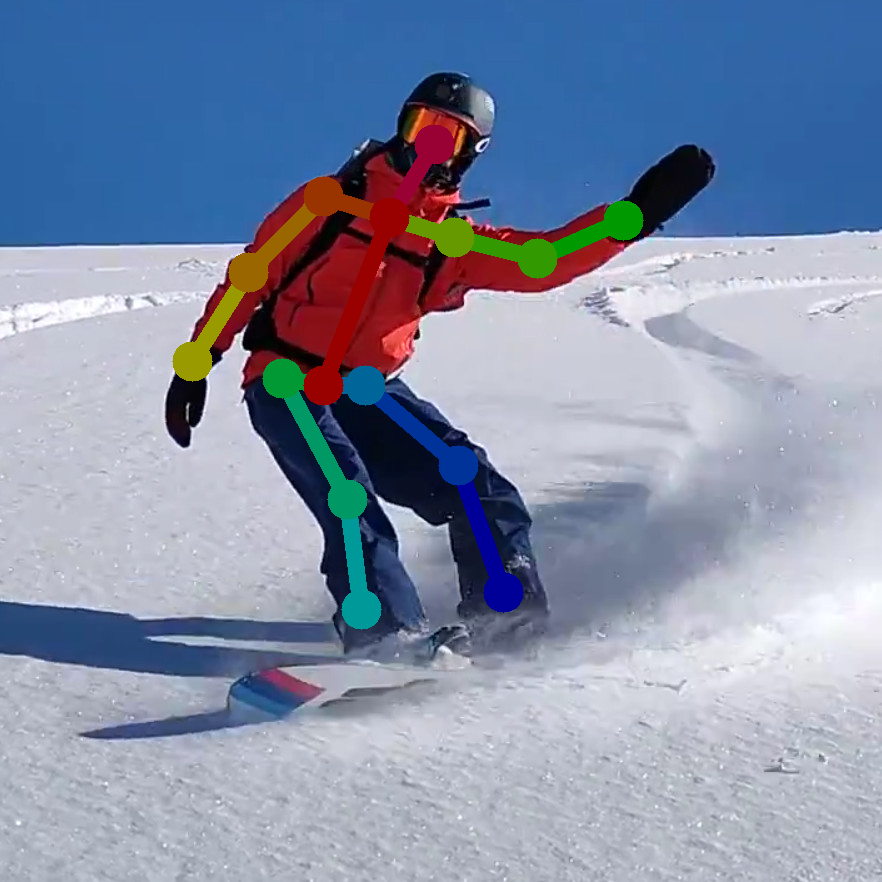
\includegraphics[width=1\linewidth]{images/board.png}
    \caption{The human pose overlaid over the input image}
    \label{fig:board}
  \end{subfigure}
  \hspace{2em}
  \begin{subfigure}[t]{.45\textwidth}
    \center
    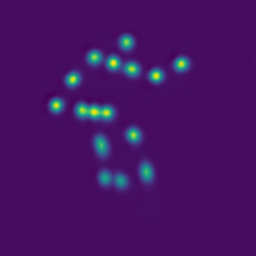
\includegraphics[width=1\linewidth]{images/board_conf.png}
    \caption{The confidence map the direct output of the neural network}
    \label{fig:conf}
  \end{subfigure}
  \caption{}
  \end{figure}
  \begin{itemize}
    \item Porting from the \texttt{Python}-API to the \texttt{C++}-API
      \item Adding multiperson HPE with Part Affinity Fields as presented in \cite{cao_simon_wei_sheikh_2017}
      \begin{itemize}
          \item  Implementation in \texttt{C++} and \texttt{HLS}
      \end{itemize}
      \item Removing the person in the image and only dispaly the human pose
      \begin{itemize}
        \item Simple approaches like, paint an human avatar over the person
          \item Classical computer vision Image Inpainting approaches like \cite{criminisi_perez_toyama_2004}
          \begin{itemize}
              \item \texttt{HLS}
          \end{itemize}
          \item With modern deep learning \cite{nazeri_ng_joseph_qureshi_ebrahimi_2019}
          \begin{itemize}
              \item Vitis AI
          \end{itemize}
      \end{itemize}
  \end{itemize}

  
  \bibliography{references}{}
  \bibliographystyle{ieeetr}


\end{document}